\documentclass[12pt,a4paper]{article}
\usepackage[utf8]{inputenc}
\usepackage[spanish]{babel}
\usepackage{amsmath}
\usepackage{amsfonts}
\usepackage{amssymb}
\usepackage{graphicx}
\usepackage[left=2cm,right=2cm,top=2cm,bottom=2cm]{geometry}

\usepackage{enumitem}
\usepackage{algorithm}
\usepackage{algorithmic}
\usepackage[hidelinks]{hyperref}

\usepackage{subcaption}
\usepackage{pgfplots}

% Para la tabla
\usepackage[normalem]{ulem}
\useunder{\uline}{\ul}{}


\author{Ignacio Aguilera Martos}
\title{Práctica 1 \\ Aprendizaje Automático}
\date{25 de Marzo de 2019}

\setlength{\parindent}{0cm}
\setlength{\parskip}{10px}


\begin{document}
	\maketitle

	\tableofcontents

	\newpage

\section{Ejercicio 1}

\subsection{Apartado 1}

Se nos pide implementar el algoritmo de gradiente descendente, veamos como funciona para justificar la implementación.

El algoritmo de gradiente descendente aplicado a minimización de funciones toma la idea del ajuste de una función lineal que hemos estudiado en teoría. Ahora en vez de actualizar $w_j$ de forma proporcional a la derivada parcial j-ésima de el error dentro de la muestra vamos a actualizarla mediante la derivada parcial j-ésima de la función que queremos minimizar.

El algoritmo parte de un punto $w$ inicial, que se irá actualizando hasta aproximar el mínimo de la función. El valor de $w$ en la iteración i+1-ésima será el valor de $w$ en la iteración i-ésima menos una constante de proporcionalidad que llamamos tasa de aprendizaje por el gradiente de la función a minimizar, esto es:

$$w_{i+1} = w_i - \eta \cdot \nabla f(x_1,...,x_n)$$

Donde $f(x_1,...,x_n)$ es la función que queremos minimizar.

De esta forma lo que vamos a hacer en la práctica es comprobar lo siguiente: vamos a actualizar de esta forma el valor de $w$ hasta que agotemos un número de iteraciones máximas fijadas o hasta que el valor absoluto de la diferencia de $f(w_i)$ y $f(w_{i+1})$ sea menor que una cierta tolerancia, esto es que la imagen de los $w_i$ y $w_{i+1}$ no hayan experimentado un cambio apreciable entre dos iteraciones consecutivas.

Cabe destacar que en mi caso he generalizado la implementación del algoritmo mediante el uso de la librería SymPy. Mediante esta librería he implementado una función que generaliza el cálculo del gradiente en un punto, de tal forma que no tengo que programar explícitamente la función que calcula el gradiente de la función que queremos minimizar. Esto se plasma en las funciones ``evaluate'' y ``gradiente'' de mi código.

\subsection{Apartado 2}

\subsubsection{Apartado a}

En este apartado se nos proporciona la siguiente función a minimizar:

$$E(u,v) = (u^2 e^{v} - 2v^2 e^{-u})^2$$

Vamos a calcular analíticamente la expresión del gradiente como se nos pide en el ejercicio. Lo primero que tenemos que hacer es ver cómo sería la expresión del gradiente en nuestro caso:

$$\nabla E(u,v) = (\frac{\partial E(u,v)}{\partial u},\frac{\partial E(u,v)}{\partial v})$$

Calculemos pues cada una de las dos parciales.

$$\frac{\partial E(u,v)}{\partial u} = 2(u^2 e^{v} - 2v^2 e^{-u})(2ue^{v}+2v^2e^{-u})$$

$$\frac{\partial E(u,v)}{\partial v} = 2(u^2 e^{v} - 2v^2 e^{-u})(u^2 e^{v}-4ve^{-u})$$

Por tanto:

$$\nabla E(u,v) = (\frac{\partial E(u,v)}{\partial u},\frac{\partial E(u,v)}{\partial v}) = 2 (u^2 e^{v} - 2v^2 e^{-u})\cdot [(2ue^{v}+2v^2e^{-u}), (u^2 e^{v}-4ve^{-u})](u,v)$$

Cabe decir que esta es una función $\nabla E(u,v): \mathbb{R}^2 \rightarrow \mathbb{R}^2$, es decir que toma dos variables y que obtiene un vector de dimensión 2.

\subsubsection{Apartado b y c}

En este apartado se nos pide dar el punto en el que el método de gradiente descendente ha alcanzado por primera vez un valor de la función menor que $10^{-14}$ y el número de iteraciones que ha consumido hasta obtener dicho valor.

En este caso el punto en el que se ha encontrado un valor que cumple esta restricción es $w=(0.619207678450638,0.968448269010049)$ y para ello ha consumido $33$ iteraciones.

\subsection{Apartado 3}

Consideramos en este apartado la función:

$$f(x,y) = x^2 + 2y^2 + 2\sin{(2\pi x)}\sin{(2\pi y)}$$

\subsubsection{Apartado a}

Se nos pide aplicar el algoritmo de gradiente descendente a la función anteriormente definida empezando en el punto $(x_0 = 0.1, y_0 = 0.1)$ con tasa de aprendizaje $\eta = 0.01$ y como máximo $50$ iteraciones.

Tras esto se nos pide elaborar un gráfico con los valores de la función obtenidos para cada iteración. Veamos los gráficos para poder analizarlos.

\begin{figure}[H]
	\centering
	\begin{subfigure}{0.45\textwidth}
		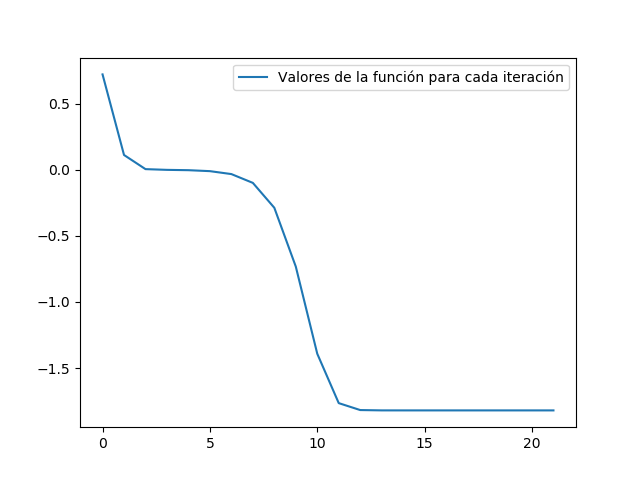
\includegraphics[scale=0.5]{./Imagenes/3a1.png}
		\caption{Tasa de aprendizaje $\eta=0.01$}
		\label{3a1}
	\end{subfigure}
	\begin{subfigure}{0.45\textwidth}
		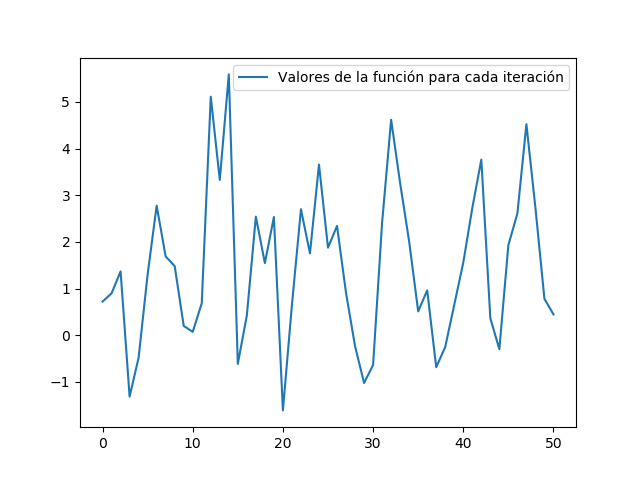
\includegraphics[scale=0.5]{./Imagenes/3a2.png}
		\caption{Tasa de aprendizaje $\eta=0.1$}
		\label{3a2}
	\end{subfigure}
\end{figure}

Como podemos observar el resultado usando $\eta=0.01$ siempre mejora en cada iteración, o a lo sumo permanece en un valor igual, en cambio con $\eta=0.1$ obtenemos una oscilación pronunciada entre iteraciones, esto es, entre dos iteraciones consecutivas no siempre pasamos a un punto con menor valor de la función, si no que mejoramos y empeoramos el resultado de forma cíclica.

Cabe explicar este comportamiento de forma más detallada para razonarlo. La tasa de aprendizaje nos da el factor de salto por el que va multiplicado el gradiente de la función, es decir, a mayor tasa de aprendizaje mayor será el salto que hagamos para obtener el siguiente valor de $w$. Supongamos que tenemos una función como $f(x)=x^2$:

\begin{figure}[H]
	\centering
	\begin{tikzpicture}
		\begin{axis}[ 
			xlabel=$x$,
			ylabel={$f(x) = x^2$}
			] 
			\addplot[blue,thick](x,x^2); 
		\end{axis}
	\end{tikzpicture}
\end{figure}

Según el valor de la tasa de aprendizaje $\eta$ podemos encontrarnos con los dos escenarios que nos están ocurriendo:

\begin{figure}[H]
	\begin{subfigure}{0.45\textwidth}
		\centering
		\begin{tikzpicture}
			\begin{axis}[ 
				xlabel=$x$,
				ylabel={$f(x) = x^2$}
				] 
				\addplot[blue,thick](x,x^2);
				\addplot+ [mark=*] table{
					0 0
					-2 4
					-4 16
				};
			\end{axis}
		\end{tikzpicture}
	\end{subfigure}
	\begin{subfigure}{0.45\textwidth}
		\centering
		\begin{tikzpicture}
		\begin{axis}[ 
		xlabel=$x$,
		ylabel={$f(x) = x^2$}
		] 
		\addplot[blue,thick](x,x^2);
		\addplot+ [mark=*] table{
			0 0
			1 1
			-1 1
			2 4
			-2 4
			3 9
			-3 9
			4 16
			-4 16
		};
		\end{axis}
		\end{tikzpicture}
	\end{subfigure}
	\caption{Ejemplo de comportamiento del gradiente descendente}
	\label{descripcionEta}
\end{figure}

Como podemos ver una aproximación no realiza ``saltos'' alrededor del mínimo, si no que va de forma directa al mínimo, mientras que en el otro caso tenemos una oscilación alrededor del mínimo. 

Si estudiamos la dependencia del comportamiento del algoritmo en función de la tasa de aprendizaje $\eta$ vemos que la magnitud del salto del punto actual al siguiente viene dada exactamente por $\eta$ en la dirección del gradiente de la función.

En nuestro caso, con $\eta = 0.01$ podemos observar en la gráfica \textbf{\ref{3a1}} que la convergencia es de forma gradual y sin saltos alrededor del mínimo, pues siempre que se progresa en cada iteración se hace obteniendo un valor menor de la función, es decir estaríamos en el primero de los casos expuestos de la figura \textbf{\ref{descripcionEta}}.

En el segundo caso con $\eta=0.1$ podemos observar en la gráfica \textbf{\ref{3a2}} que el comportamiento es errático. Si observamos la evolución entre iteraciones podemos observar que no mejora si no que oscila alrededor del mínimo sin llegar a él. Esto es debido a que la longitud del salto, es decir, el valor de $\eta$ es demasiado grande y hace que avance demasiado entre iteraciones. Esto comparado con nuestro ejemplo de la figura \textbf{\ref{descripcionEta}} se correspondería con el segundo de los casos, en el que el camino hacia el mínimo de la función se hace oscilando entorno a él.

En la figura con $\eta=0.1$ también se aprecia que la amplitud de valores que toma va disminuyendo, es decir, poco a poco se está dirigiendo hacia el mínimo. El algoritmo gradiente descendente llegará eventualmente al mínimo con este valor de $\eta$ pero consumirá un número mucho mayor de iteraciones que si escogemos de forma más ajustada la tasa de aprendizaje.

Esto último mencionado no quiere decir que el algoritmo partiendo de un punto inicial fijo siempre converja hacia el mismo mínimo de la función, ya que puede que en función del valor de $\eta$ las iteraciones vayan saltando hasta dar con otro mínimo local o global de la función.

\subsubsection{Apartado b}

Se nos pide obtener el valor mínimo con 50 iteraciones fijando los puntos de inicio $w_1 = (0.1,0.1)$, $w_2 = (1,1)$, $w_3 = (-0.5,-0.5)$, $w_4 = (-1,-1)$.

Veamos los valores mínimos obtenidos con estos puntos:

\begin{table}[H]
	\begin{tabular}{|l|c|l|}
		\hline
		{\textbf{Punto inicial}} & {\textbf{Mínimo encontrado}}            & {\textbf{Valor en el mínimo}} \\ \hline \hline
		{[}0.1 0.1{]}                & {[}0.243804966858502 -0.237925820555452{]}  & -1.82008                          \\ \hline
		{[}1 1{]}                    & {[}1.21807029968290 0.712811949619077{]}    & 0.593269                          \\ \hline
		{[}-0.5 -0.5{]}              & {[}-0.731377457654812 -0.237855363313347{]} & -1.33248                          \\ \hline
		{[}-1 -1{]}                  & {[}-1.21807029968290 -0.712811949619077{]}  & 0.593269                          \\ \hline
	\end{tabular}
\end{table}

Como podemos observar el punto de inicio es altamente determinante para obtener el mínimo de la función ya que dependiendo del valor inicial podemos acabar obteniendo uno u otro mínimo local o incluso el mínimo global de la función. Como podemos ver inclusive en esta función (por ciertas razones de simetría de los senos) hemos acabado obteniendo como mínimo un punto y su opuesto como se puede ver en las filas 2 y 4 de la tabla.

\subsection{Apartado 4}

Si observamos todos los resultados que hemos obtenido hasta ahora podemos obtener dos conclusiones acerca de la dificultad de hallar un mínimo:

\begin{itemize}
	\item La elección de la tasa de aprendizaje: si escogemos una tasa de aprendizaje muy grande podemos incluso forzar que la convergencia se produzca en un número de iteraciones excesivamente grande no obteniendo por tanto un mínimo satisfactorio de la función. Esto no es realmente un problema, puesto que siempre podemos escoger una tasa de aprendizaje muy pequeña para avanzar en pasos pequeños y no saltarnos el mínimo más próximo al punto de inicio. Esto nos obligaría probablemente a usar un número mayor de iteraciones, pero no influiría en el mínimo que obtenemos.
	\item El punto de inicio: esto es totalmente determinante. Supongamos que tenemos una función con una serie de mínimos locales y un mínimo global de la siguiente forma:
	\begin{figure}[H]
		\centering
		\begin{tikzpicture}
			\begin{axis}[ 
			xlabel=$x$,
			ylabel={$f(x) = \frac{x^6}{6} - \frac{17x^4}{2} + \frac{225x^2}{2}$}
			] 
			\addplot[domain=-6:6,blue,thick,smooth,samples=1000]{(1/6)*x^6 - (1/2)*17*x^4 + (1/2)*225*x^2};
			\addplot+ [mark=*,thick,red] table{
				-5.5 238.534
			};
			\addplot+ [mark=*,thick,orange] table{
				2 324.667
			};
			\addplot+ [mark=*,thick,black] table{
				4 306.667
			};
			\end{axis}
		\end{tikzpicture}
	\end{figure}
	Si consideramos como punto de partida el punto rojo con una tasa de aprendizaje adecuada acabaremos llegando al mínimo local que tiene justo a su derecha, gracias a que el gradiente de la función  ``empuja'' al algoritmo hacia ese punto. 
	
	Si tomásemos como punto inicial el punto negro iríamos también hacia el mínimo local que tiene a su derecha.
	
	En cambio estos dos mínimos no son los mínimos globales de la función ya que de los tres puntos tomados sólo el naranja tendería hacia el mínimo real de la función. En este caso es fácil poder escoger el punto inicial del que partimos, incluso en una función de dos variables sería sencillo tomar este punto inicial pero imaginemos una función de 10 variables con valores en $\mathbb{R}$. Esta función ya no la podemos dibujar, por lo que no podemos tomar el punto de forma visual aproximada. Si no tenemos más información sobre la función este es el paso más complejo del algoritmo pues según nuestra elección del punto inicial obtendremos un verdadero mínimo global (si es que existe) o un mínimo local de la función.
\end{itemize}

\section{Ejercicio 2}
\subsection{Apartado 1}
\subsubsection{Algoritmos}
Vamos en primer lugar a estudiar los algoritmos que se nos proponen para implementar.

El primero de los algoritmos implementados es el algoritmo de la pseudo inversa. Este algoritmo se basa en la resolución del método de mínimos cuadrados lineal, es decir, resolver el problema de ajustar una serie de datos mediante una función lineal minimizando el cuadrado de los errores a dicha función. Esto se puede visualizar con ejemplos clásicos como:

\begin{figure}[H]
	\centering
	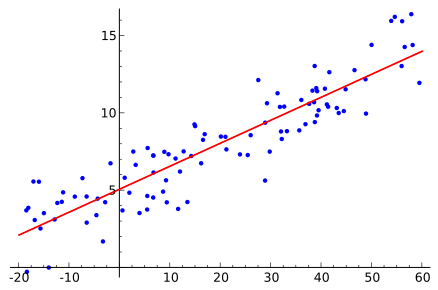
\includegraphics[scale=0.7]{./Imagenes/ej2-1.png}
	\caption{Ejemplo de la función lineal con mínimos cuadrados.}
	\label{ej2-1}
\end{figure}

en la cual podemos intuir que la recta minimiza los errores entre los valores de la propia recta y los valores reales de los puntos del conjunto de datos.

El fundamento teórico parte de que podemos expresar el gradiente de $E_{in}(w)$ como:

$$\nabla E_{in}(w) = \frac{2}{N}X^T (Xw - y) = 0$$

De donde podemos obtener la aproximación de igualdad $X^T X w = X^T y$

Entonces podemos expresar $w$ como $w = X^{\dagger}y$ donde $X^{\dagger} = (X^T X)^{-1}X^T$

Pero no tenemos la certeza de que podamos calcular siempre $(X^T X)^{-1}$, por lo que acudimos a lo que se define como la pseudo inversa de Moore-Penrose.

Partimos de la descomposición en valores singulares de la matriz $X = UDV^T$, entonces podemos obtener que $X^TX = VDDV^T$.

Si intentamos obtener la inversa de aquí entonces obtenemos $(X^TX)^{-1} = (V^T)^{-1}(D^2)^{-1}V^T$. Observemos que D sí es una matriz invertible pues contiene los valores singulares no nulos de $X$ y por tanto tiene determinante no nulo.

Visto ya todo esto sólo resta volver al punto anterior a la disertación sobre la inversa y ver que podemos definir $X^{\dagger} = (X^T X)^{-1}X^T$. Con este comportamiento es con el que se ha implementado el algoritmo de la pseudo inversa.

Para gradiente descendente estocástico partimos de la base conocida del algoritmo gradiente descendente aplicado a regresión lineal.

La idea es la misma que en el algoritmo gradiente descendente. Queremos actualizar el valor de $w$ en función de un factor $\eta$ que llamamos tasa de aprendizaje y en función de $\frac{\partial E_{in}(w)}{\partial w_j}$, pero en este caso no tenemos en cuenta toda la muestra completa, si no que vamos a crear subconjuntos de la muestra que llamamos ``minibatches''. Estos subconjuntos tienen un tamaño finito, típicamente entre 32 y 128 (en mi implementación particular 64 por recomendación del profesor del prácticas).

Por tanto el valor de $w$ lo vamos a actualizar tomando, como se muestra en las diapositivas de teoría:

$$\frac{\partial E_{in}(w)}{\partial w_j} = \frac{2}{M}\sum_{n=1}^{M}x_{nj}(h(x_n)-y_n)$$

Donde M es el tamaño del minibatch y tomamos los índices correspondientes al mismo para el cómputo del cálculo. Es decir, tomando la filosofía de gradiente descendente tendríamos:

$$w_j = w_j - \eta \frac{\partial E_{in}(w)}{\partial w_j}$$

Por tanto el algoritmo recibirá un número de iteraciones, para cada una de las cuales calcularemos una secuencia de índices de donde obtendremos los minibatches y actualizaremos el valor de $w$ tal y como acabamos de describir. Cada una de estas iteraciones es normalmente llamada época.

\subsubsection{Resultados}

Tal y como describe el enunciado he empleado los dos algoritmos (pseudo inversa y gradiente descendente estocástico) para obtener las rectas que separan los datos de las dos clases existentes.

Veamos por tanto el resultado obtenido pintando el conjunto de datos por clases y las rectas obtenidas según los dos algoritmos:

\begin{figure}[H]
	\centering
	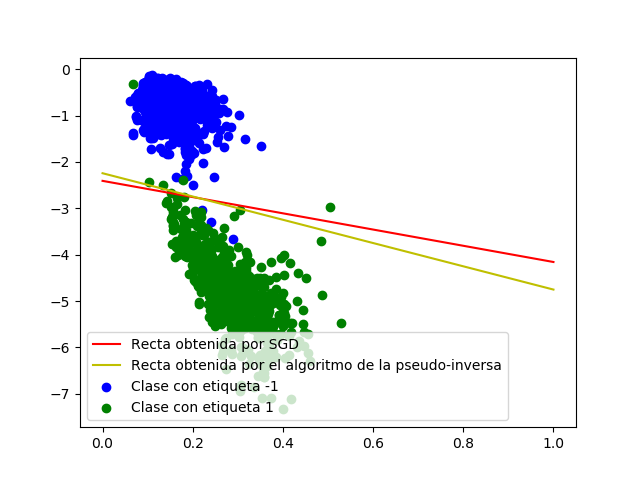
\includegraphics[scale=0.8]{./Imagenes/ej2-1_w.png}
	\caption{Rectas obtenidas por SGD y el algoritmo de la pseudo inversa}
	\label{ej2-1_w}
\end{figure}

Como podemos observar ambas rectas son buenas fronteras de los conjuntos dados por cada clase, ya que ambas delimitan (o se encuentran cerca de la idea de frontera de los conjuntos) de forma aceptable los conjuntos de diferentes clases.

Además si observamos los errores obtenemos los siguientes datos:

\begin{table}[H]
	\begin{tabular}{|l|l|l|}
		\hline
		& \textbf{Gradiente Descendente Estocástico} & \textbf{Pseudo Inversa}      \\ \hline \hline
		$\mathbf{E_{in}}$  & 0.07953827330086667               & 0.07918658628900395 \\ \hline
		$\mathbf{E_{out}}$ & 0.1319506351366829               & 0.13095383720052572 \\ \hline
	\end{tabular}
\end{table}

De donde podemos observar que el algoritmo de la pseudo inversa funciona ligeramente mejor que el algoritmo de gradiente descendente estocástico, al menos para los parámetros elegidos para este algoritmo. En este caso he tomado como $\eta = 0.01$ y 1000 iteraciones. Esta tasa de aprendizaje la he tomado atendiendo a diferentes pruebas que he realizado. Se puede observar que a partir de valores no mucho mayores a 0.01 el algoritmo no converge adecuadamente y con valores menores a 0.01 se actualiza el valor de $w$ demasiado lento, por lo que he convenido usar 0.01.

Podemos ver que tanto para el error dentro de la muestra, esto es usando los datos de train del conjunto proporcionado como para el error fuera de la muestra, es decir usando los datos de test del conjunto proporcionado obtenemos un error menor en el algoritmo de la pseudo inversa. Podemos intuir, que al aumentar el número de iteraciones de GDS obtendremos un mejor resultado que el algoritmo de la pseudo inversa. Este hecho intuitivo viene dado por la realidad de que el algoritmo de la pseudo inversa siempre nos da el mismo resultado, mientras que SGD va mejorando el valor obtenido a mayor número de iteraciones dadas.

Podemos ver además que el algoritmo SGD va mejorando a cada iteración el error dentro de la muestra ($E_{in}$):
\begin{figure}[H]
	\centering
	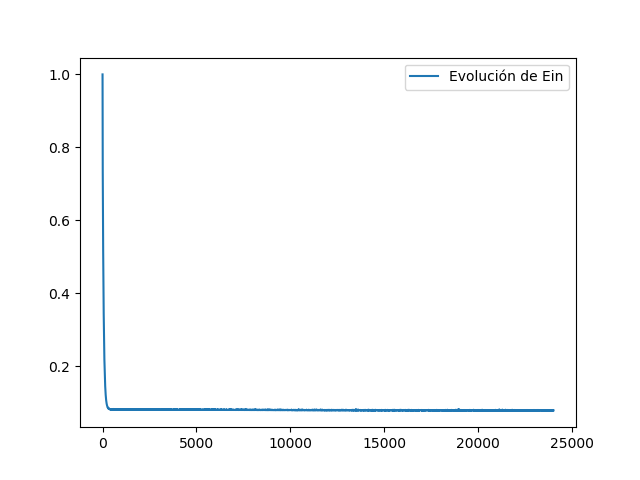
\includegraphics[scale=0.8]{./Imagenes/ej2-1_evol_ein.png}
	\caption{Evolución del error dentro de la muestra para SGD}
	\label{ej2-1_evol_ein}
\end{figure}
aunque como se puede percibir, la mejora en el error disminuye de forma notable a partir de la iteración 300 aproximadamente.

Como añadido a los resultados, cabe explicar cómo he representado la recta. Los puntos del conjunto de datos son de la forma $(1,x,y)$ y son multiplicados por $w^T$, veamos entonces la ecuación de la recta obtenida:

$$w^T(1,x,y) = (w_1,w_2,w_3)^T(1,x,y) = w_1 + w_2\cdot x + w_3\cdot y = 0$$

Despejando la y obtenemos $y = \frac{-w_1 - w_2\cdot x}{w_3}$. Ahora observemos que podemos pintar la recta por ejemplo entre los puntos 0 y 1, para ello tenemos que ver por dónde pasa la recta por estos puntos, es decir, sustituir x por 0 y por 1. De esta forma obtendremos dos puntos por los que pasa la recta y por tanto dos puntos por donde podremos pasar la función plot de matplotlib. Estos puntos serán $(0,\frac{-w_1}{w_3})$ y $(1,\frac{-w_1 - w_2}{w_3})$.

\subsection{Apartado 2}
Lo primero que se nos pide en el experimento es que muestreemos 1000 puntos en el espacio 2-dimensional $[-1,1]\times [-1,1]$ mediante una distribución uniforme. Veamos la nube de puntos generada:

\begin{figure}[H]
	\centering
	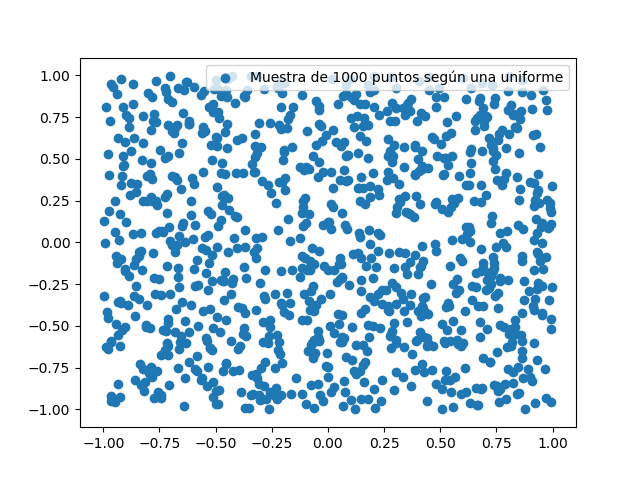
\includegraphics[scale=0.7]{./Imagenes/ej2-2-1.png}
	\caption{Nube de puntos muestreada}
	\label{ej2-2-1}
\end{figure}

Como se puede ver, los puntos están uniformemente distribuidos en el cuadrado $[-1,1]\times [-1,1]$.

Ahora hemos considerado la función $f(x_1,x_2) = sign((x_1-0.2)^2 + x_{2}^{2}-0.6)$ la cual hemos usado para obtener etiquetas de cada punto, con lo que obtendremos etiquetas 1 y -1. Veamos la distribución de los puntos por clase:

\begin{figure}[H]
	\centering
	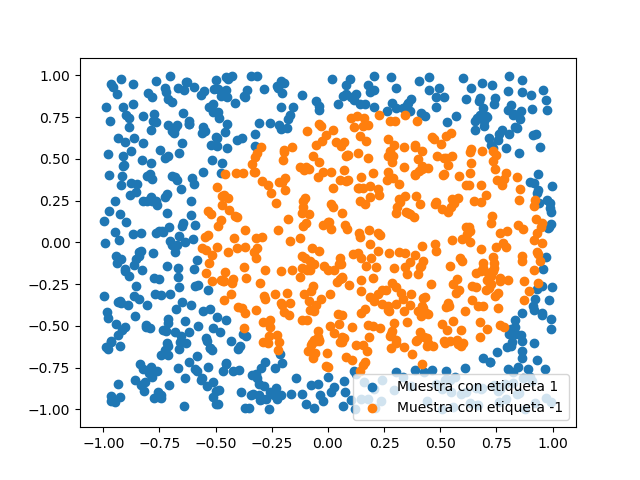
\includegraphics[scale=0.8]{./Imagenes/ej2-2-3.png}
	\caption{Muestra uniforme por clases en función de f}
	\label{ej2-2-3}
\end{figure}

Como podemos observar la geometría del conjunto de datos es difícil de ajustar mediante una transformación lineal, de hecho sabemos que la frontera del conjunto tiene forma cuadrática y por ello presumiblemente al obtener la frontera mediante una función lineal el error será alto en este ejemplo.

Tras esto debemos introducir ruido en el conjunto, es decir, cambiar a la etiqueta opuesta al $10\%$ de puntos de conjunto, de donde obtenemos el conjunto de datos siguiente:

\begin{figure}[H]
	\centering
	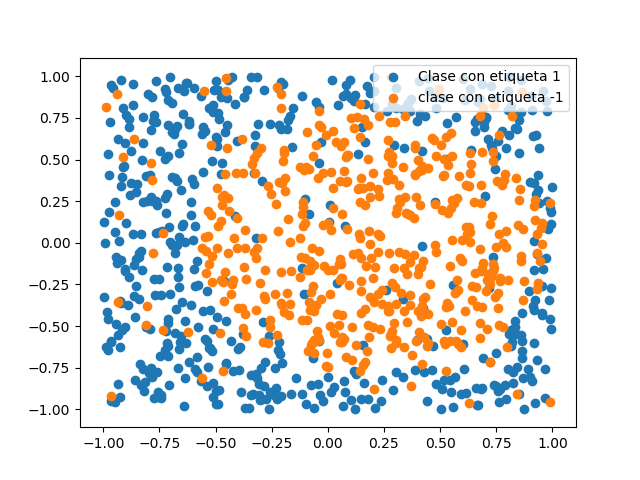
\includegraphics[scale=0.8]{./Imagenes/ej2-2-2.png}
	\caption{Conjunto de datos después de añadirle ruido}
	\label{ej2-2-2}
\end{figure}

Como podemos observar la tendencia general de los datos sigue siendo la distribución en una  transformación no lineal (cuadrática) y ahora con algunos puntos mas mezclados entre las clases por culpa del 10\% añadido con el ruido.

Usando este conjunto de datos obtenemos un error de $E_{in} = 0.9285857795136097$ y $E_{out} = 0.8900691837207613$ que es bastante elevado. Observemos en la figura el por qué de este error tan alto:

\begin{figure}[H]
	\centering
	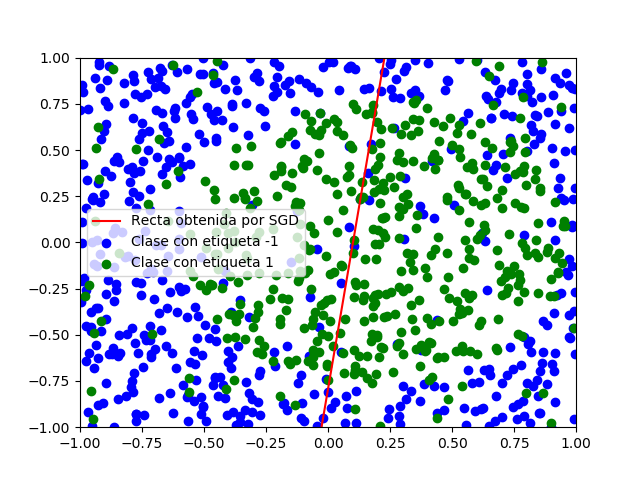
\includegraphics[scale=0.8]{./Imagenes/ej2-2-4.png}
	\caption{Recta obtenida para la muestra}
	\label{ej2-2-4}
\end{figure}

Como podemos ver la separación no es nada satisfactoria pues deja muchos puntos mezclados.

Ahora el experimento se repite haciendo 1000 veces esta generación aleatoria uniforme, produciendo el ruido e intentando ajustar la función lineal que separa los datos por etiquetas. Veamos la media de los errores en el experimento han sido $E_{in} = 0.9268179758401789$ y $E_{out} = 0.8973487193216161$. Como podemos observar la tendencia no es del ejemplo concreto descrito anteriormente, si no que en media, en este tipo de conjuntos, el comportamiento de las transformaciones lineales no es satisfactorio.

\section{Bonus}
El algoritmo implementado para el ejercicio bonus es el algoritmo de Newton o Método de Newton. En el algoritmo de gradiente descendente empleamos como aproximación el gradiente de la función de la que queríamos obtener el mínimo. Este hecho viene determinado de que el gradiente nos da la tendencia o dirección del cambio de una función. En análisis multivariante o análisis de varias variables la Hessiana cuenta con un papel muy relevante también a la hora del estudio de los puntos de mínimo y máximo valor de una función de varias variables. En concreto, por ejemplo, sabemos que si la función tiene Hessiana definida positiva, entonces la función cuenta con un mínimo en el punto en el que se produzca la convexidad. Veamos la forma de la matriz hessiana en general para nuestra función $f(x_1,x_2)$ de dos variables:

$$Hess(f) = \begin{pmatrix}
\frac{\partial^2 f(x_1,x_2)}{\partial x_{1}^{2}} & \frac{\partial^2 f(x_1,x_2)}{\partial x_1 \partial x_2} \\
\frac{\partial^2 f(x_1,x_2)}{\partial x_2 \partial x_1} & \frac{\partial^2 f(x_1,x_2)}{\partial x_{2}^{2}} \\
\end{pmatrix}$$

Veamos de dónde proviene la idea de usar la matriz hessiana. Para empezar debemos saber qué son los polinomios de Taylor. Estos polinomios, explicados de forma simple, son polinomios que aproximan una función mediante una suma infinita de términos de la forma $f(x) = \sum_{n=0}^{\infty}\frac{f^{(n)}(a)}{n!}(x-a)^n$. Este polinomio nos da la forma para aquellas funciones que son de una sola variable. El concepto se puede extender a funciones de varias variables, pero como es evidente ya no podemos hacer la derivada n-ésima si no que debemos generalizarlo con el gradiente, la hessiana y derivadas de orden superior. En particular la hessiana nos aparece en el segundo término de esta expansión de Taylor y por tanto podemos pensar que una forma de aproximar la función puede ser empleando la hessiana.

Se puede probar, aunque no es de relevancia en este estudio pues se desconecta demasiado de la asignatura, que el gradiente y la hessiana mantienen una cierta relación. Es este hecho el que nos lleva a pensar que el gradiente de la función empleado en el método de gradiente descendente es sustituible por la hessiana.

Una vez motivada la aparición de la hessiana vamos a ver cómo funciona el algoritmo.

Al igual que en gradiente descendente vamos a modificar w a cada paso de la siguiente forma:

$$w_{n+1} = w_n-\eta Hess(f(x_1,x_2))^{-1}\nabla f(x_1,x_2)$$

Donde $w_{n+1}$ representa el valor de $w$ en la iteración n+1-ésima y $w_n$ representa el valor de $w$ en la iteración n-ésima.

Esta actualización de la variable dependiente del gradiente y la hessiana no es de extrañar dado que ya hemos motivado que mantienen una relación entre sí y ambos elementos (el gradiente y la hessiana) aparecen en el desarrollo de la función mediante polinomios de Taylor.

Veamos cómo ha funcionado este algoritmo con las mismas iteraciones que gradiente descendente en el primer ejercicio (50 iteraciones) y con los mismos puntos de inicio comparando los valores de función obtenidos en los mínimos encontrados.

\begin{table}[H]
	\begin{tabular}{|l|c|l|}
		\hline
		{\textbf{Punto inicial}} & {\textbf{Mínimo encontrado}}            & {\textbf{Valor en el mínimo}} \\ \hline \hline
		{[}0.1 0.1{]}                & {[}0.0486405155671848 0.0483402069479654{]}  & 0.187016232200131                          \\ \hline
		{[}1 1{]}                    & {[}0.980088999815528 0.990265537884792{]}    & 2.93708035581126                          \\ \hline
		{[}-0.5 -0.5{]}              & {[}-0.490075759559880 -0.495162184791504{]} & 0.734333236339149                          \\ \hline
		{[}-1 -1{]}                  & {[}-0.980088999815528 -0.990265537884792{]}  & 2.93708035581126                          \\ \hline
	\end{tabular}
\end{table}

Si los comparamos con los obtenidos en gradiente descendente podemos ver que en todos los casos el resultado dado por el método de Newton es peor. Veamos por qué estudiando cómo descienden las gráficas de los valores de la función a lo largo de las iteraciones:

\begin{figure}[H]
	\begin{subfigure}{0.24\textwidth}
		\centering
		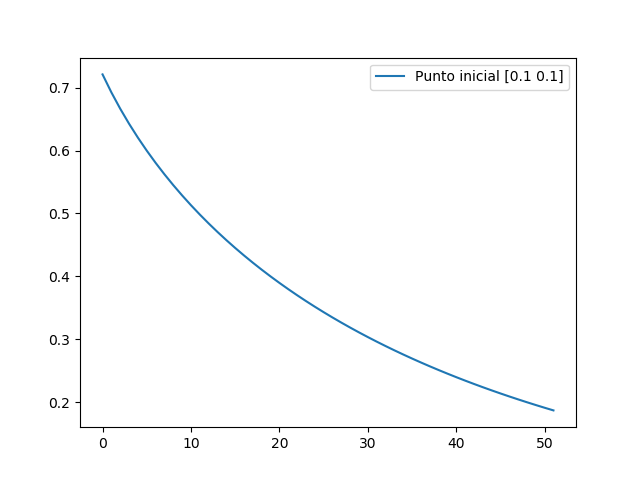
\includegraphics[scale=0.3]{./Imagenes/bonus1.png}
	\end{subfigure}
	\begin{subfigure}{0.24\textwidth}
		\centering
		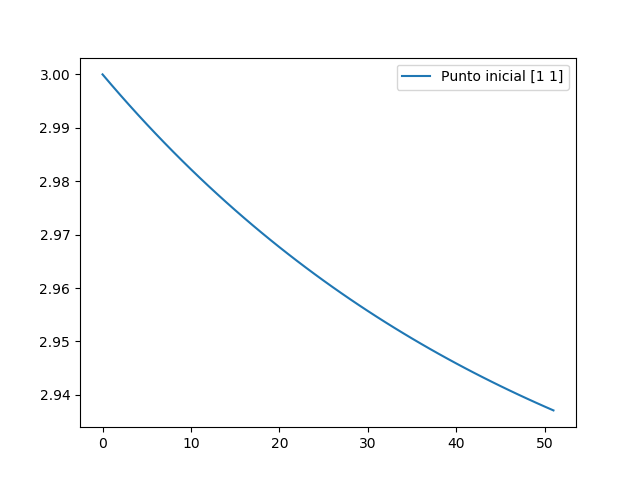
\includegraphics[scale=0.3]{./Imagenes/bonus2.png}
	\end{subfigure}
	\begin{subfigure}{0.24\textwidth}
		\centering
		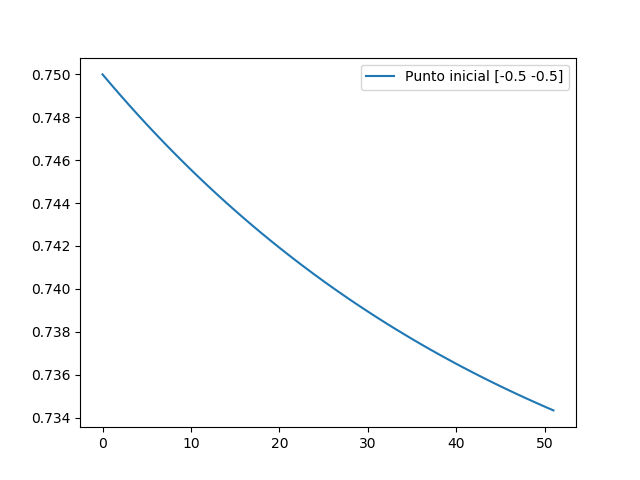
\includegraphics[scale=0.3]{./Imagenes/bonus3.png}
	\end{subfigure}
	\begin{subfigure}{0.24\textwidth}
		\centering
		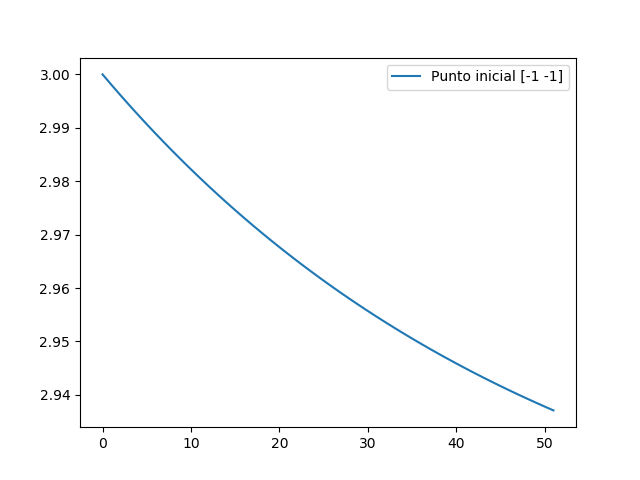
\includegraphics[scale=0.3]{./Imagenes/bonus4.png}
	\end{subfigure}
	\caption{Convergencia de los valores de la función con el método de Newton}
	\label{convergenciaNewton}
\end{figure}

Aquí podemos ver que la convergencia es mucho más lenta que en el caso de gradiente descendente, podemos ver que comparado con la función que muestra el valor de la función a cada iteración en el empleo de gradiente descendente y en este caso con el método de Newton tenemos un comportamiento mucho más lento con el método de Newton. 

Este hecho es el que nos ha llevado a la obtención de peores resultados, pues a mismo número de iteraciones el algoritmo de gradiente descendente consigue mejor resultado que el método de Newton.

Si por contra consideramos ahora $\eta=0.1$ obtenemos resultados mejores pero que siguen sin ser tan satisfactorios como los que nos proporciona gradiente descendente, veamos los resultados obtenidos:

\begin{table}[H]
	\begin{tabular}{|l|c|l|}
		\hline
		{\textbf{Punto inicial}} & {\textbf{Mínimo encontrado}}            & {\textbf{Valor en el mínimo}} \\ \hline \hline
		{[}0.1 0.1{]}                & {[}0.000331244760829602 0.000327706859870783{]}  & 8.89535208376675e-6                          \\ \hline
		{[}1 1{]}                    & {[}0.949380622715943 0.974700533836422{]}    & 2.90040704776242                          \\ \hline
		{[}-0.5 -0.5{]}              & {[}-0.475230636355934 -0.487862825996409{]} & 0.725482618291771                          \\ \hline
		{[}-1 -1{]}                  & {[}-0.949380622715943 -0.974700533836422{]}  & 2.90040704776242                          \\ \hline
	\end{tabular}
\end{table}

En el ámbito que si hemos mejorado es en el de la convergencia como podemos ver en las gráficas de convergencia:

\begin{figure}[H]
	\begin{subfigure}{0.24\textwidth}
		\centering
		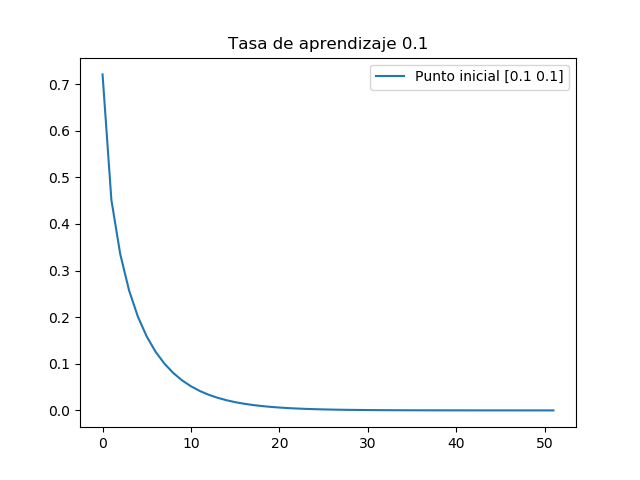
\includegraphics[scale=0.3]{./Imagenes/bonus8.png}
	\end{subfigure}
	\begin{subfigure}{0.24\textwidth}
		\centering
		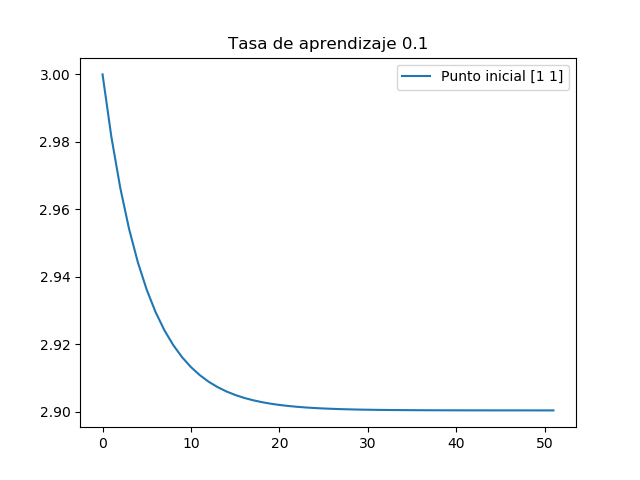
\includegraphics[scale=0.3]{./Imagenes/bonus9.png}
	\end{subfigure}
	\begin{subfigure}{0.24\textwidth}
		\centering
		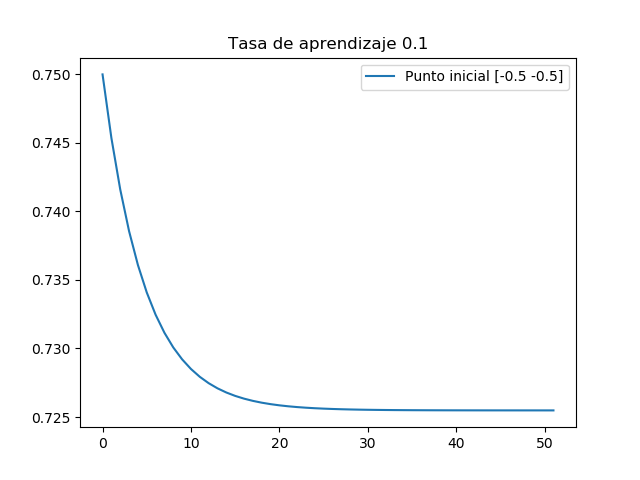
\includegraphics[scale=0.3]{./Imagenes/bonus10.png}
	\end{subfigure}
	\begin{subfigure}{0.24\textwidth}
		\centering
		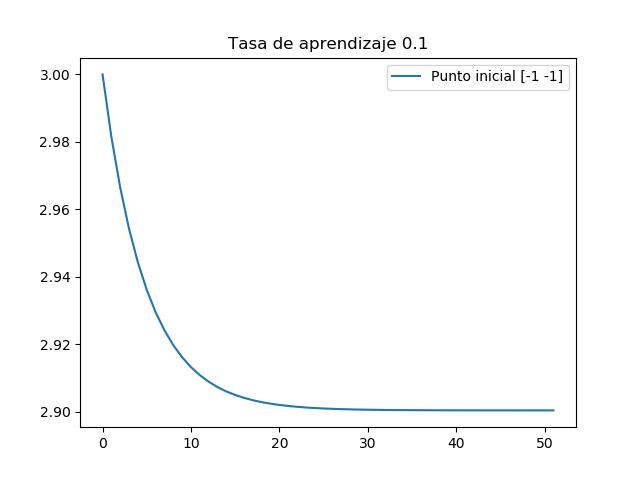
\includegraphics[scale=0.3]{./Imagenes/bonus11.png}
	\end{subfigure}
	\caption{Convergencia de los valores de la función con el método de Newton}
	\label{convergenciaNewton2}
\end{figure}

Esto no quiere decir que siempre sea mejor el uso de gradiente descendente. Pudiéramos encontrar una función en la que el mínimo fuera localizado de forma más eficiente por el método de Newton debido a que su avance es más lento que el que nos da el método de gradiente descendente. Visualicemos por ejemplo esta función:

\begin{figure}[H]
	\centering
	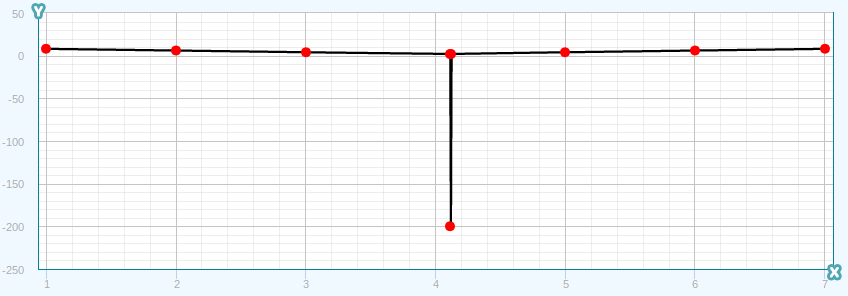
\includegraphics[scale=0.5]{./Imagenes/bonus5.png}
	\caption{Ejemplo de función para el método de Newton}
	\label{bonus5}
\end{figure}

Como podemos ver esta función tiene un mínimo muy claro pero concentrado en un punto muy concreto de la función. El método de Newton nos proporciona de por sí (a misma tasa de aprendizaje) un avance más lento que gradiente descendente. Este hecho podría ser aprovechado para detectar mínimos de este tipo en funciones pues es más fácil hacer que el método de Newton caiga en este mínimo que lo haga el algoritmo de gradiente descendente a misma tasa de aprendizaje.

Cabe decir que el método de Newton funciona bien cuando la matriz hessiana es definida positiva, esto ocurre (aplicando el llamado criterio de Sylvester) cuando los menores principales de la matriz tienen determinante positivo. Esto en nuestro caso particular se traduce en que $\frac{\partial^2 f(x_1,x_2)}{\partial x_{1}^{2}}>0$ y que el determinante de la matriz hessiana sea positivo. Esto no ocurre en todo punto, es decir, existen conjuntos de puntos donde la matriz hessiana no es definida positiva. Bajo estas condiciones se sabe que el método de Newton converge a puntos de silla y no a mínimos, tal y como nos está ocurriendo. Visualicemos este comportamiento con $\eta=0.01$:

\begin{figure}[H]
	\centering
	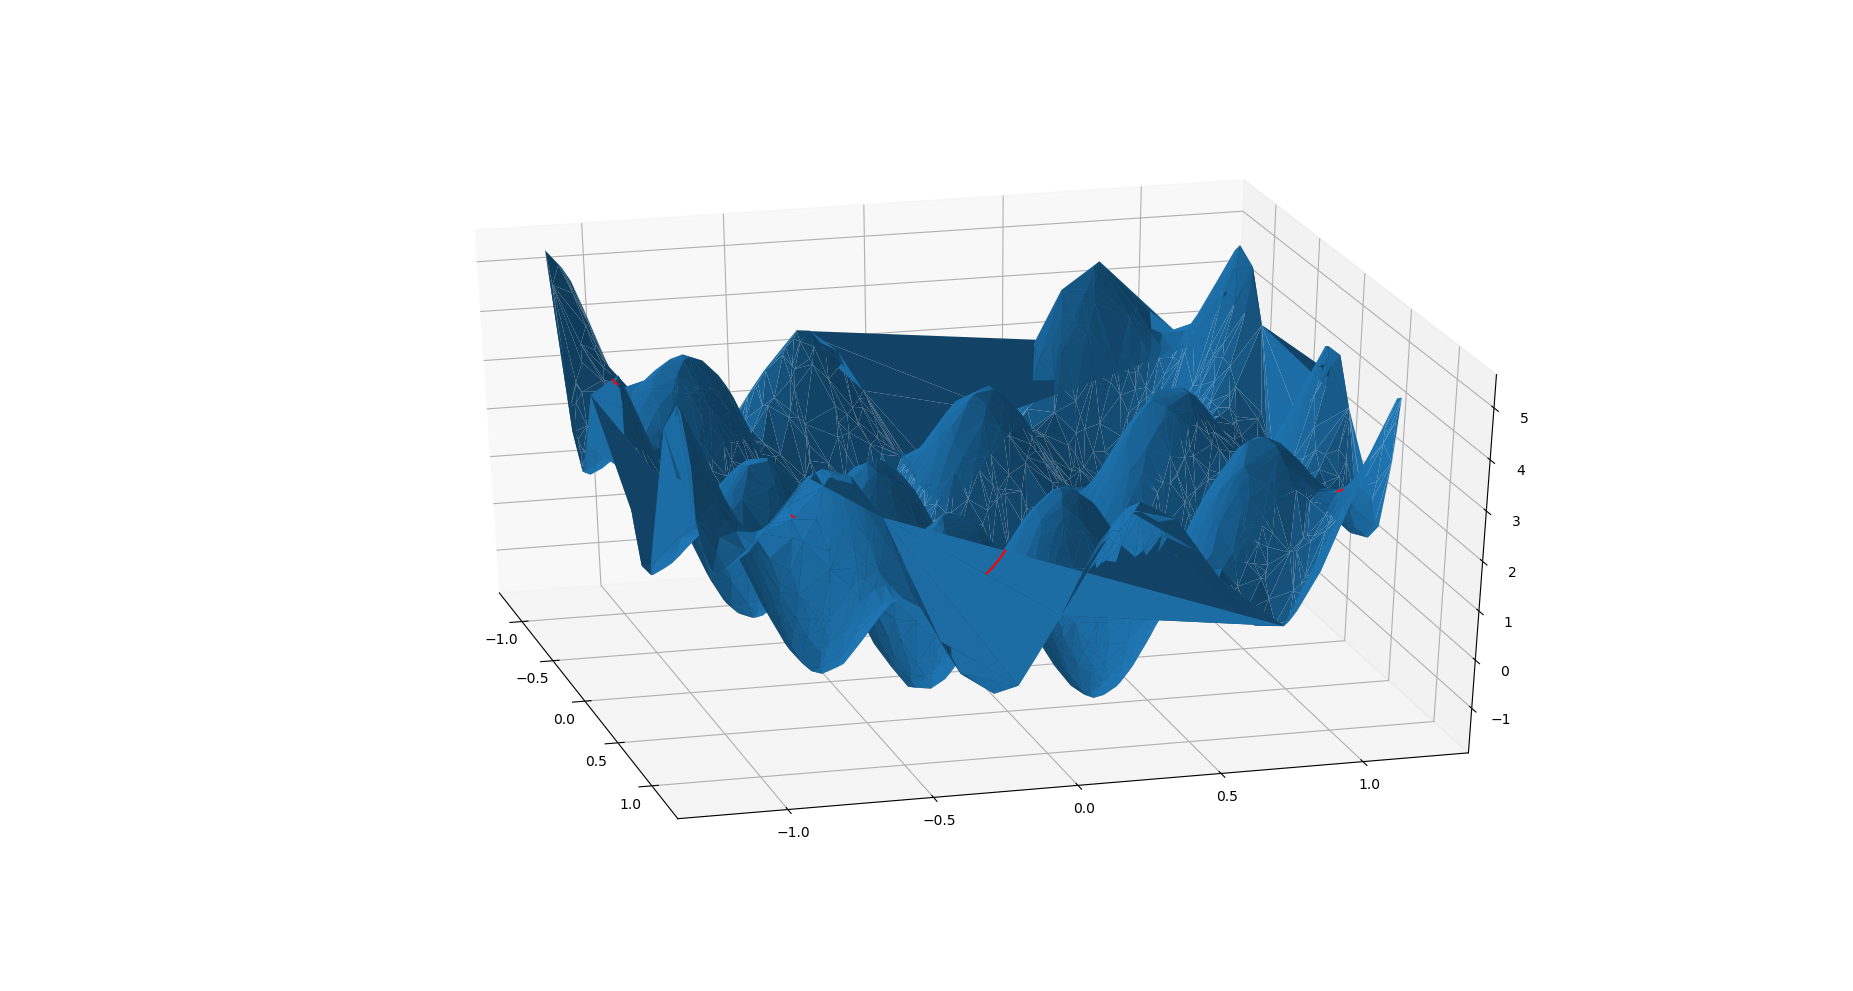
\includegraphics[scale=0.4]{./Imagenes/bonus6.png}
	\caption{Movimiento descrito por el algoritmo de Newton desde el lateral con $\eta=0.01$}
\end{figure}

\begin{figure}[H]
	\centering
	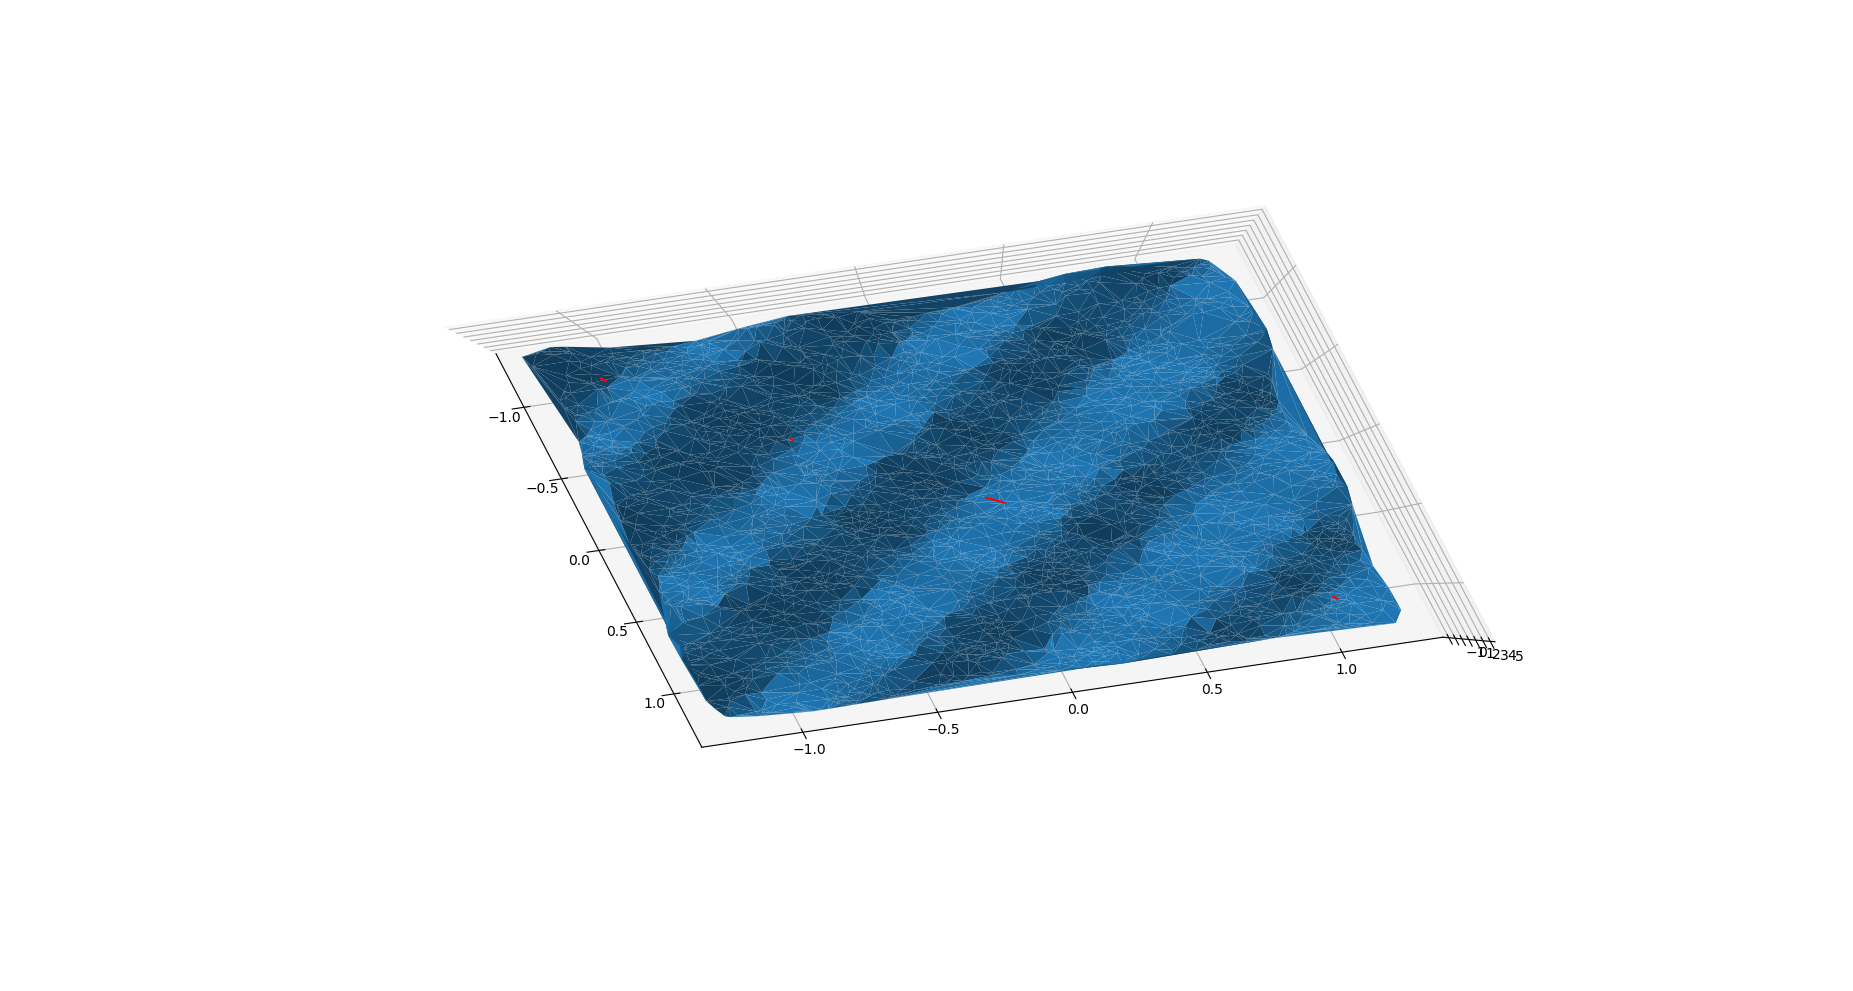
\includegraphics[scale=0.4]{./Imagenes/bonus7.png}
	\caption{Movimiento descrito por el algoritmo de Newton desde arriba con $\eta=0.01$}
\end{figure}

\begin{figure}[H]
	\centering
	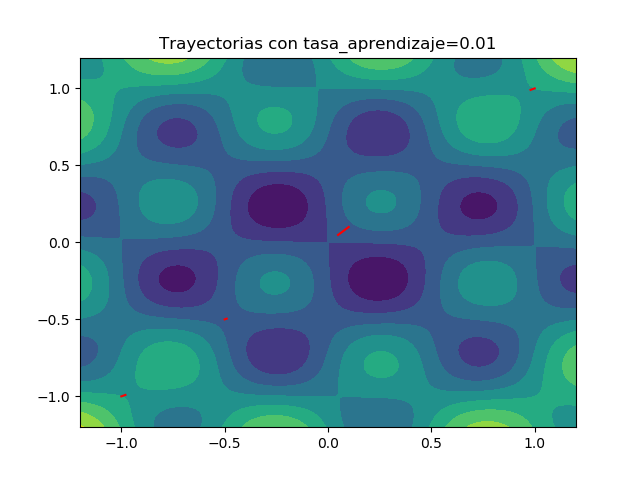
\includegraphics[scale=0.8]{./Imagenes/bonus12.png}
	\caption{Trayectorias con $\eta=0.01$}
\end{figure}

Veamos que  esto no cambia cuando $\eta=0.1$:

\begin{figure}[H]
	\centering
	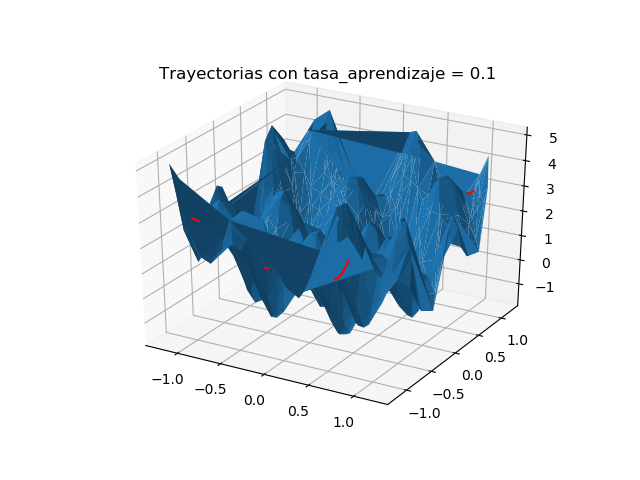
\includegraphics[scale=0.8]{./Imagenes/bonus14.png}
	\caption{Movimiento descrito por el algoritmo de Newton desde el lateral con $\eta=0.1$}
\end{figure}

\begin{figure}[H]
	\centering
	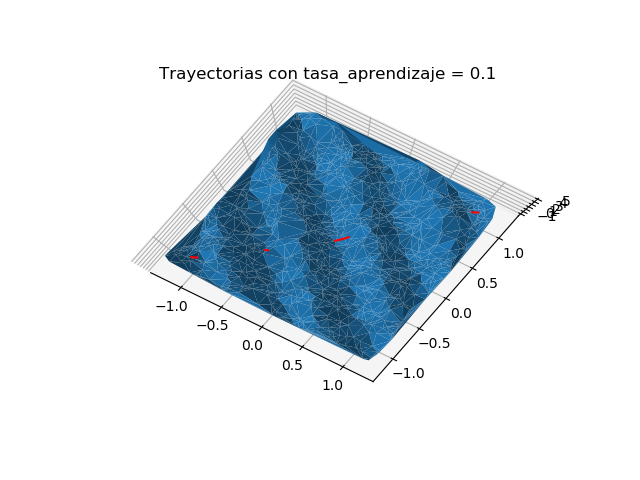
\includegraphics[scale=0.8]{./Imagenes/bonus15.png}
	\caption{Movimiento descrito por el algoritmo de Newton desde arriba con $\eta=0.1$}
\end{figure}

\begin{figure}[H]
	\centering
	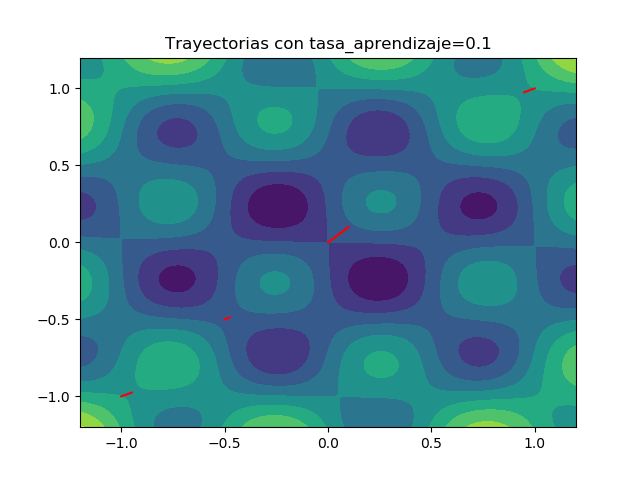
\includegraphics[scale=0.8]{./Imagenes/bonus13.png}
	\caption{Trayectorias con $\eta=0.1$}
\end{figure}

Como podemos observar el comportamiento es exactamente el que la teoría nos predijo, converge a puntos de silla en vez de mínimos debido a que la matriz hessiana no es definida positiva.

La ventaja que presenta el algoritmo de Newton frente a gradiente descendente es que, bajo condiciones de convexidad, esto es que la hessiana sea definida positiva, la convergencia del algoritmo de Newton es cuadrática (más rápido que lo que nos proporciona gradiente descendente). De esta forma una estrategia bajo la cual podría ser útil emplear el algoritmo de Newton sería utilizar un algoritmo como gradiente descendente en la primera fase de la ejecución para poder utilizar en la última el algoritmo de Newton. Si la primera fase acaba con un punto cercano a un mínimo el algoritmo de Newton se lanzará con velocidad cuadrática hacia él ajustando mucho más rápido el valor mínimo que gradiente descendente.

\end{document}
